\documentclass[10pt,aspectratio=149]{beamer}

% All the boilerplate is in ac1slides.sty
% Note that this also pulls in a custom vogtwidebar.sty
\usepackage{ac1slides}

\author{Ji\v{r}\'i Lebl}

\institute[OSU]{%
Departemento pri Matematiko de Oklahoma {\^S}tata Universitato}

\title{BA: 7.3}

\date{}

\begin{document}

\begin{frame}
\titlepage
\end{frame}

\begin{frame}
\begin{definition}
A \emph{sequence} in a metric space $(X,d)$ is a function
$x \colon \N \to X$.
\pause
Write $x_n$ for the $n$th element.
\pause
For the whole sequence write
\begin{equation*}
\{ x_n \}_{n=1}^\infty .
\end{equation*}
\pause
$\{ x_n \}_{n=1}^\infty$ is \emph{bounded} if
$\exists$ $p \in X$ and $B \in \R$ such that
\begin{equation*}
d(p,x_n) \leq B \qquad \text{for all } n \in \N.
\end{equation*}
\pause
That is, $\{x_n\}_{n=1}^\infty$ is bounded \wiffif
$\{ x_n : n \in \N \}$ is bounded.

\pause
\medskip

If $\{ n_k \}_{k=1}^\infty$ is a sequence of natural numbers
such that $n_{k+1} > n_k$ for all $k$,

then $\{ x_{n_k} \}_{k=1}^\infty$
is a \emph{subsequence} of $\{x_n \}_{n=1}^\infty$.
\end{definition}

\end{frame}

\begin{frame}

\begin{definition}
$\{ x_n \}_{n=1}^\infty$ in a metric space $(X,d)$ is said
to \emph{converge} to 
$p \in X$ if

for every $\epsilon > 0$, there exists an $M \in \N$ such
that $d(x_n,p) < \epsilon$ for all $n \geq M$.

\pause
\medskip

$p$
is said to be a \emph{limit}
of $\{ x_n \}_{n=1}^\infty$.

\pause
\medskip

If the limit is unique, write
\quad $\displaystyle
\lim_{n\to \infty} x_n \coloneqq p$.

\pause
\medskip

A sequence that converges is \emph{convergent}.

\pause
Otherwise, the sequence is \emph{divergent}.
\end{definition}

\pause
\medskip

\begin{center}
\scalebox{0.8}{
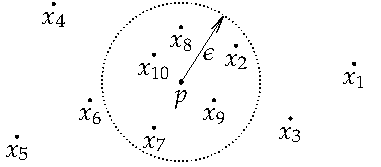
\includegraphics{../figures/sequence-convergence-metric}
}
\end{center}

Sequence converging to $p$.  The first 10 points 
are shown and $M=7$ for this $\epsilon$.

\end{frame}

\begin{frame}

\begin{proposition}
A convergent sequence in a metric space has a unique limit.
\end{proposition}

\pause
\textbf{Remark:} Proof is exactly the same as for real-sequences.

\pause
\medskip

\textbf{Proof:}
Suppose $\{ x_n \}_{n=1}^\infty$ has limits $x$ and $y$.

\pause
Take an arbitrary $\epsilon > 0$.

\pause
Find an $M_1$ such that for all $n \geq M_1$,
\quad
$d(x_n,x) < \nicefrac{\epsilon}{2}$.


\pause
Find an $M_2$ such that for all $n \geq M_2$,
\quad
$d(x_n,y) < \nicefrac{\epsilon}{2}$.

\pause
Consider $n$ such that $n \geq M_1$ \textbf{and} $n \geq M_2$.

\pause
$
d(y,x)
\pause
\leq
d(y,x_n)+d(x_n,x)
\pause
<
\frac{\epsilon}{2} + \frac{\epsilon}{2} = \epsilon .
$

\pause
$d(y,x) < \epsilon$ $\forall$  $\epsilon > 0$ \wthus $d(y,x) = 0$
\pause
\wthus $y=x$.

\pause
Hence the limit (if it exists) is unique.
\qed

\end{frame}

\begin{frame}

\begin{proposition}
A convergent sequence in a metric space is bounded.
\end{proposition}

\pause
\begin{proposition}
A sequence $\{ x_n \}_{n=1}^\infty$ in a metric space $(X,d)$ converges to $p \in X$
if and only
if there exists a sequence $\{ a_n \}_{n=1}^\infty$ of real numbers such that
\begin{equation*}
d(x_n,p) \leq a_n \quad \text{for all } n \in \N,
\qquad
\text{and}
\qquad
\lim_{n\to\infty} a_n = 0.
\end{equation*}
\end{proposition}

\pause
\begin{proposition}
Let $\{ x_n \}_{n=1}^\infty$ be a sequence in a metric space $(X,d)$.
\begin{enumerate}[(i)]
\item
\pause
If $\{ x_n \}_{n=1}^\infty$ converges to $p \in X$, then every
subsequence $\{ x_{n_k} \}_{k=1}^\infty$
converges to $p$.
\item
\pause
If for some $K \in \N$ the $K$-tail $\{ x_n \}_{n=K+1}^\infty$
converges to $p \in X$, then
 $\{ x_n \}_{n=1}^\infty$ converges to $p$.
\end{enumerate}
\end{proposition}

\pause
\textbf{Proofs:} Exercises.

\end{frame}

%\begin{frame}
%
%\textbf{Example:}
%Take $C\bigl([0,1],\R\bigr)$ be the set of continuous functions with the metric being
%the uniform metric.  We saw that we obtain a metric space.
%If we look at the definition of convergence, we notice that it is identical
%to uniform convergence.  That is, $\{ f_n \}_{n=1}^\infty$ converges uniformly if and only
%if it converges in the metric space sense.
%
%\medskip
%
%\textbf{Remark:}
%It is perhaps surprising that on the set of functions $f \colon [a,b] \to
%\R$ (continuous or not)
%there is no metric that gives pointwise convergence.  Although the proof of
%this fact is beyond the scope of this book.
%
%\end{frame}

\begin{frame}

\begin{proposition}
Consider $\{ x_m \}_{m=1}^\infty$ in $\R^n$,
where $x_m = \bigl(x_{m,1},x_{m,2},\ldots,x_{m,n}\bigr) \in \R^n$.
\pause
Then,

 $\{ x_m \}_{m=1}^\infty$ converges \wiffif
$\{ x_{m,k} \}_{m=1}^\infty$ converges for every $k=1,2,\ldots,n$,

\medskip
\pause
in which case
\qquad
$\displaystyle
\lim_{m\to\infty}
x_m =
\Bigl(
\lim_{m\to\infty} x_{m,1},
\lim_{m\to\infty} x_{m,2},
\ldots,
\lim_{m\to\infty} x_{m,n}
\Bigr) .
$
\end{proposition}

\pause

\textbf{Proof:}
Suppose
$\{ x_m \}_{m=1}^\infty$ converges to
$y = (y_1,y_2,\ldots,y_n) \in \R^n$.

\pause
\medskip

Given $\epsilon > 0$, $\exists$ $M$ such that $\forall$ $m \geq M$, ~~
$d(y,x_m) < \epsilon$.

\pause
\medskip

Fix some $k=1,2,\ldots,n$.

\pause
For all $m \geq M$,
\begin{equation*}
\bigl\lvert y_k - x_{m,k} \bigr\rvert
\pause
=
\sqrt{{\bigl(y_k - x_{m,k} \bigr)}^2}
\pause
\leq
\sqrt{\sum_{\ell=1}^n {\bigl(y_\ell-x_{m,\ell}\bigr)}^2}
\pause
= d(y,x_m) < \epsilon .
\end{equation*}
\pause
\thus \quad $\{ x_{m,k} \}_{m=1}^\infty$ converges to $y_k$.

\end{frame}

\begin{frame}

Now suppose
$\{ x_{m,k} \}_{m=1}^\infty$ converges to $y_k$ for every $k=1,2,\ldots,n$.

\pause
\medskip

Given $\epsilon > 0$, pick $M$ such that $\forall$ $m \geq M$ and
$\forall$ $k = 1,\ldots,n$, ~~
$\bigl\lvert y_k-x_{m,k} \bigr\rvert < \nicefrac{\epsilon}{\sqrt{n}}$.
\pause
\begin{equation*}
d(y,x_m)
\pause
=
\sqrt{\sum_{k=1}^n {\bigl(y_k-x_{m,k}\bigr)}^2}
\pause
<
\sqrt{\sum_{k=1}^n {\left(\frac{\epsilon}{\sqrt{n}}\right)}^2}
\pause
=
\sqrt{\sum_{k=1}^n \frac{{\epsilon^2}}{n}}
\pause
= \epsilon .
\end{equation*}
\pause
\thus \quad
$\{ x_m \}_{m=1}^\infty$ converges to
$y = (y_1,y_2,\ldots,y_n) \in \R^n$.
\qed

%\end{frame}

%\begin{frame}

\pause
\bigskip

\textbf{Example:}
In the set of complex numbers $\C$, $z = x+iy$,

\pause
$\{ z_n \}_{n=1}^\infty = \{ x_n + iy_n \}_{n=1}^\infty$ converges
to $z = x+iy$

\pause
\wiffif

$\{ x_n \}_{n=1}^\infty$ converges to $x$
and 
$\{ y_n \}_{n=1}^\infty$ converges to $y$.

\end{frame}

\begin{frame}

\begin{proposition}
Let $(X,d)$ be a metric space and $\{x_n\}_{n=1}^\infty$ a sequence in $X$.  Then
$\{ x_n \}_{n=1}^\infty$ converges to $p \in X$ if and only if for every open neighborhood
$U$ of $p$, there exists an $M \in \N$ such that for all $n \geq M$,
we have $x_n \in U$.
\end{proposition}

\pause
\textbf{Proof:}
Suppose $\{ x_n \}_{n=1}^\infty$ converges to $p$.

\pause
Let $U$ be an open neighborhood of $p$.

\pause
\thus \quad $\exists$ $\epsilon > 0$ such that $B(p,\epsilon) \subset U$.

\pause
Find $M \in \N$ such that $\forall$ $n \geq M$, ~~ $d(p,x_n) < \epsilon$,
\pause
~~that is,~~ $x_n \in B(p,\epsilon) \subset U$.

\pause
\medskip

The other direction:

\pause
Given $\epsilon > 0$, let $U \coloneqq B(p,\epsilon)$ be the neighborhood of $p$.

\pause
\thus \quad $\exists$ $M \in \N$
such that for $n \geq M$, ~~ $x_n \in U = B(p,\epsilon)$,

\pause
that is, ~~ $d(p,x_n) < \epsilon$.
\qed

\end{frame}

\begin{frame}

\begin{proposition}
Let $(X,d)$ be a metric space, $E \subset X$ a closed set,
and $\{ x_n \}_{n=1}^\infty$ a sequence in $E$ that converges to some $p \in X$.
Then $p \in E$.
\end{proposition}

\pause
\textbf{Proof:}
We prove the contrapositive.

\pause
\medskip

Suppose $\{ x_n \}_{n=1}^\infty$ in $X$ converges to $p \in E^c$.

\pause
\medskip

$E^c$ is open
\pause
\wthus
$\exists$
$M$ such that $\forall$ $n \geq M$,~
$x_n \in E^c$.

\pause
\medskip

\thus \quad $\{ x_n \}_{n=1}^\infty$ is not a sequence in $E$.
\qed

\end{frame}

\begin{frame}

\begin{proposition}
Let $(X,d)$ be a metric space and $A \subset X$.
Then $p \in \widebar{A}$ if and only if there exists a sequence
$\{ x_n \}_{n=1}^\infty$ of
elements in $A$ such that $\lim\limits_{n\to\infty} x_n = p$.
\end{proposition}

\pause
\textbf{Proof:}
Let $p \in \widebar{A}$.

\pause
\medskip

For every $n \in \N$,
~ $\exists$
$x_n \in B(p,\nicefrac{1}{n}) \cap A$.

\pause
\medskip

$d(p,x_n) < \nicefrac{1}{n}$ $\forall n$
\pause
\wthus
$\lim_{n\to\infty} x_n = p$.

\pause
\medskip

The other direction: Exercise.
\qed

\end{frame}

\begin{frame}

\textbf{Exercise:}
Let $(X,d)$ be a metric space where $d$ is the discrete metric.  Suppose 
$\{ x_n \}_{n=1}^\infty$ is a convergent sequence in $X$.  Show that there exists
a $K \in \N$ such that for all $n \geq K$, we have $x_n = x_K$.

\pause
\medskip

A set $S \subset X$ is said to be \emph{dense} in $X$ if
$X \subset \widebar{S}$ or in other words if for every $p \in X$,
there exists a sequence $\{ x_n \}_{n=1}^\infty$ in $S$ that converges to $p$.

\pause
\medskip

\textbf{Exercise:}
Prove that $\R^n$ contains a countable dense subset.

\pause
\medskip

\textbf{Exercise:}
Let $(X,d)$ be a metric space and $\{ x_n \}_{n=1}^\infty$ a sequence in $X$.
Prove that $\{ x_n \}_{n=1}^\infty$ converges to $p \in X$
if and only if
every subsequence of $\{ x_n \}_{n=1}^\infty$ has a subsequence that
converges to $p$.

\end{frame}

\end{document}
